%%%%%%%%%%%%%%%%%%%%%%%%%%%%%%%%%%%%%%%%%
% Beamer Presentation
% LaTeX Template
% Version 1.0 (10/11/12)
%
% This template has been downloaded from:
% http://www.LaTeXTemplates.com
%
% License:
% CC BY-NC-SA 3.0 (http://creativecommons.org/licenses/by-nc-sa/3.0/)
%
%%%%%%%%%%%%%%%%%%%%%%%%%%%%%%%%%%%%%%%%%

%----------------------------------------------------------------------------------------
%	PACKAGES AND THEMES
%----------------------------------------------------------------------------------------

\documentclass{beamer}

\mode<presentation> {

% The Beamer class comes with a number of default slide themes
% which change the colors and layouts of slides. Below this is a list
% of all the themes, uncomment each in turn to see what they look like.

%\usetheme{default}
%\usetheme{AnnArbor}
%\usetheme{Antibes}
%\usetheme{Bergen}
%\usetheme{Berkeley}
%\usetheme{Berlin}
%\usetheme{Boadilla}
%\usetheme{CambridgeUS}
\usetheme{Copenhagen}
%\usetheme{Darmstadt}
%\usetheme{Dresden}
%\usetheme{Frankfurt}
%\usetheme{Goettingen}
%\usetheme{Hannover}
%\usetheme{Ilmenau}
%\usetheme{JuanLesPins}
%\usetheme{Luebeck}
%\usetheme{Madrid}
%\usetheme{Malmoe}
%\usetheme{Marburg}
%\usetheme{Montpellier}
%\usetheme{PaloAlto}
%\usetheme{Pittsburgh}
%\usetheme{Rochester}
%\usetheme{Singapore}
%\usetheme{Szeged}
%\usetheme{Warsaw}

% As well as themes, the Beamer class has a number of color themes
% for any slide theme. Uncomment each of these in turn to see how it
% changes the colors of your current slide theme.

%\usecolortheme{albatross}
%\usecolortheme{beaver}
%\usecolortheme{beetle}
%\usecolortheme{crane}
\usecolortheme{dolphin}
%\usecolortheme{dove}
%\usecolortheme{fly}
%\usecolortheme{lily}
%\usecolortheme{orchid}
%\usecolortheme{rose}
%\usecolortheme{seagull}
%\usecolortheme{seahorse}
%\usecolortheme{whale}
%\usecolortheme{wolverine}

%\setbeamertemplate{footline} % To remove the footer line in all slides uncomment this line
%\setbeamertemplate{footline}[page number] % To replace the footer line in all slides with a simple slide count uncomment this line

\setbeamertemplate{navigation symbols}{} % To remove the navigation symbols from the bottom of all slides uncomment this line
}

\usepackage{graphicx} % Allows including images
\usepackage{booktabs} % Allows the use of \toprule, \midrule and \bottomrule in tables
\usepackage{hyperref}

\usepackage[utf8]{inputenc}
\usepackage[spanish]{babel}
\usepackage{listings}



%----------------------------------------------------------------------------------------
%	TITLE PAGE
%----------------------------------------------------------------------------------------

\title[Busqueda Binaria Recursiva]{Algoritmo de Busqueda Binaria Recursiva} % The short title appears at the bottom of every slide, the full title is only on the title page

\author{Grupo Alias} % Your name
\institute[UTEM] % Your institution as it will appear on the bottom of every slide, may be shorthand to save space
{
Universidad Tecnológica Metropolitana\\  % Your institution for the title page
\medskip
\url{https://github.com/Lanceconan/AnalisisDeAlgoritmos} % Your site
}
\date{\today} % Date, can be changed to a custom date

\begin{document}

\setbeamercovered{transparent}

\begin{frame}
	\titlepage % Print the title page as the first slide
\begin{center}
Manuel Irarrázaval \\  Rafael Vivar \\ Daniel Gutiérrez \\ Juan Cid
\end{center}
\end{frame}

\begin{frame}
	\frametitle{Introducción} % Table of contents slide, comment this block out to remove it
	\tableofcontents % Throughout your presentation, if you choose to use \section{} and \subsection{} commands, these will automatically be printed on this slide as an overview of your presentation
\end{frame}

%----------------------------------------------------------------------------------------
%	PRESENTATION SLIDES
%----------------------------------------------------------------------------------------

%------------------------------------------------
\section{Introduccion} % Sections can be created in order to organize your presentation into discrete blocks, all sections and subsections are automatically printed in the table of contents as an overview of the talk
%------------------------------------------------

	\subsection{Definición} % A subsection can be created just before a set of slides with a common theme to further break down your presentation into chunks

		\begin{frame}
			\frametitle{Definicion}
				\begin{center}
				La búsqueda binaria en un vector ordenado de datos se realiza comprobando el elemento que está en el centro del vector y mirando si el elemento buscado es mayor o menor. 
				
				Consiste en buscar el elemento del medio (por ejemplo, si hubiera 13 elementos en la colección se comenzaría por el elemento en la 7ma posición; si hubiera 10 elementos se comienza por el que está en la 5ta posición) y comparar ese elemento por mayor o menor con respecto al elemento buscado. Si el buscado es mayor que el del medio, se descarta la mitad menor y se continúa buscando en la mitad mayor. Si es menor, se hace a la inversa. Si es igual, se ha encontrado el elemento buscado. 
				\end{center}
		
		\end{frame}

		\begin{frame}
			\frametitle{Propósito búsqueda binaria}
				
			\begin{center}
			Se utiliza cuando el vector en el que queremos determinar la existencia de un elemento está previamente ordenado.

			Este algoritmo reduce el tiempo de búsqueda considerablemente, ya que disminuye exponencialmente el número de iteraciones necesarias.
			
			Está altamente recomendado para buscar en arrays de gran tamaño. Por ejemplo, en uno conteniendo 50.000.000 elementos, realiza como máximo 26 comparaciones (en el peor de los casos).

			\end{center}
		\end{frame}


	\subsection{Funcion Binaria Recursiva en C/C++}

%------------------------------------------------

		\begin{frame}
			\frametitle{Funcion Binaria Recursiva en C/C++}
			\begin{figure}
  				\centering
    			           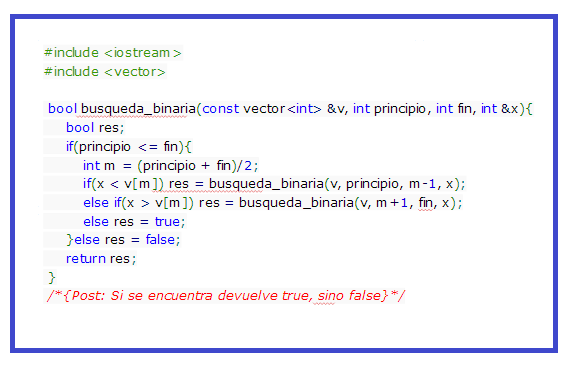
\includegraphics[scale=0.6]{CodigoC.png}
  				\caption{Codigo}
  				\label{fig:lls}
			\end{figure}
			
		\end{frame}

		
%------------------------------------------------
\section{Complejidad}
%------------------------------------------------

	\subsection{Calculo de Complejidad}

		\begin{frame}
			\frametitle{Calculo de complejidad(1)}
			Dado que este algoritmo compara el valor a buscar con el elemento central del vector presenta la siguiente ecuación de recurrencia:
			\begin{equation}
					T(n) = T(n/2) + C
				\end{equation}
			\begin{equation}
					T(1) = 1
				\end{equation}
Reemplazando las n en la ecuación original con valores sucesivos queda así:
             \begin{equation}
					T(n/2) = T(n/4) + C
				\end{equation}
				  \begin{equation}
					T(n/2) = T(n/8) + C
				\end{equation}
				  \begin{equation}
					T(n/2) = T(n/16) + C
				\end{equation}
				  \begin{equation}
					T(n/2) = T(n/32) + C
				\end{equation}
		\end{frame}


		\begin{frame}
			\frametitle{Calculo de complejidad(2)}
		Luego, se generaliza en términos de n y k para eliminar la recurrencia
			\begin{equation}
					T(n) = T(n/2) + C
				\end{equation}
			\begin{equation}
					T(n) = T(n/4) + C + C
				\end{equation}
             \begin{equation}
					T(n) = T(n/8) + C + C + C
				\end{equation}
				  \begin{equation}
					T(n) = T(n/16) + C + C + C + C
				\end{equation}
			  \begin{equation}
					T(n) = T(n/32) + C + C + C + C + C
				\end{equation}
				Resultado:
			  \begin{equation}
					T(n) = T(n/2^k) + kC
				\end{equation}
				Lo siguente es igualar con la condición inicial los términos encerrados en T(n). Pero primero, se debe despejar la variable “k”
              \begin{equation}
					n/2^k = 1 ===> n = 2^k
				\end{equation}
				
		\end{frame}
		
	

		\begin{frame}
			\frametitle{Calculo de complejidad(3)}
		Aplicando propiedades de logaritmos para despejar la variable “k”
			\begin{equation}
					log_2 {(n)} = k
				\end{equation}
		Finalmente, se procede a reemplazar los términos k con la condición inicial:
			\begin{equation}
					T(n) = T(n/2^{log_2 {(n)}}) + log_2 {(n)} * C
				\end{equation}
		Como la componente 

               \begin{equation}
                    T(n/2^{log_2 {(n)}})
                   \end{equation}


		\end{frame}


	\begin{frame}
		\frametitle{Calculo de Complejidad}
		
		 quedó igualada con la condición 

	\begin{equation}
		T(1) = 1 
	\end{equation}

	se llega al siguiente resultado
             \begin{equation}
					T(n) = 1 + log_2 {(n)} * C ===> T(n) = log_2 {(n)}
				\end{equation}
		Finalmente, se concluye que la búsqueda binaria recursiva tiene complejidad de orden
				  \begin{equation}
					O(n) = log_2 {(n)}
				\end{equation}		
	\end{frame}



%------------------------------------------------
	\subsection{Mejor y Peor Caso}

		\begin{frame}
			\frametitle{Mejor Caso}
			\begin{center}
Como en todo algoritmo (dígase de búsqueda, ordenamiento, etc.) posee su nivel de complejidad y éste no es la excepción.\\
A diferencia de la búsqueda binaria iterativa, su versión recursiva es más lenta con cada incremento de número de elementos, ya que existirán más llamadas a la función por resolver, con el consiguiente gasto de tiempo de guardar y restaurar parámetros.

			\begin{itemize}[<+->]
				\item Mejor caso: la búsqueda binaria coincide con el elemento buscado en el primer punto medio: sólo se necesitaría una comparación de elementos. Esto significa que sus tiempos de ejecución óptimos no dependen de la cantidad de datos: son constantes y por tanto proporcionales a 1, es decir, son de O(1).
				
				\item Peor caso: En el peor caso la búsqueda binaria recursiva divide el arreglo,requiriendo sólo un tiempo O(log n).
			\end{itemize}			 
			\end{center}

		\end{frame}
	

% Programa
\section{Sobre el programa}

	\subsection{Sobre el Código}
	\begin{frame}
		\frametitle{Sobre el Código}
			\begin{itemize}[<+->]
				\item IDE utilizado: Aptana Studio 3
				\item Programación en Ruby, version 1.9.3
				\item Una única clase con sus inherentes métodos
				\begin{itemize}[<+->]
					\item Métodos que permiten facil manipulación y entendimiento del código
					\item Variables Nemotécnicas
					\item Búsqueda binaria recursiva
				\end{itemize}
				\item Estructura utilizada: Un arreglo de largo N-1
				\item Metodo de Ordenamiento Burbuja (alternativo)
			\end{itemize}
	\end{frame}

	\subsection{Caracteristicas}
	\begin{frame}
		\frametitle{Caracteristicas}
			\begin{itemize}[<+->]
				\item Permite distintos poblamientos de los datos
				\begin{itemize}[<+->]
					\item Ordenado automatico (de entrada)
					\item Aleatorio
					\item Manual
				\end{itemize}
				\item Facil Manipulacion del Codigo
				\item Utiliza el ordenamiento Burbuja Complejidad 
				\begin{center}
				\begin{equation} O(n) = n^2 \end{equation} 
				\end{center}
			\end{itemize}			
	\end{frame}
	

	\subsection{Pruebas}
		
	\begin{frame}
		\frametitle{Pruebas}
			\begin{itemize}[<+->]		
				\item Peor Caso: Que el valor no esté en el vector unidimensional
					\begin{itemize}[<+->]

\item 1.000			: 10 llamados
\item10.000			: 14 llamados
\item100.000		: 17 llamados
\item1.000.000		: 20 llamados
\item10.000.000		: 24 llamados
\item100.000.000		: 27 llamados
					\end{itemize}
				
				\item Mejor Caso: Que el valor buscado está en el vector unidimensional justo en el centro estimado
					\begin{itemize}[<+->]

\item 1.000			: 1 llamado
\item 10.000			: 1 llamado
\item 100.000		: 1 llamado
\item 1.000.000		: 1 llamado
\item 10.000.000		: 1 llamado
\item 100.000.000		: 1 llamado

					\end{itemize}
			\end{itemize}

  				
	\end{frame}

	\begin{frame}
		\frametitle{Pruebas}
		\begin{figure}
			\begin{center}
				Probemos el programa 
			\end{center}
  				\centering
    			           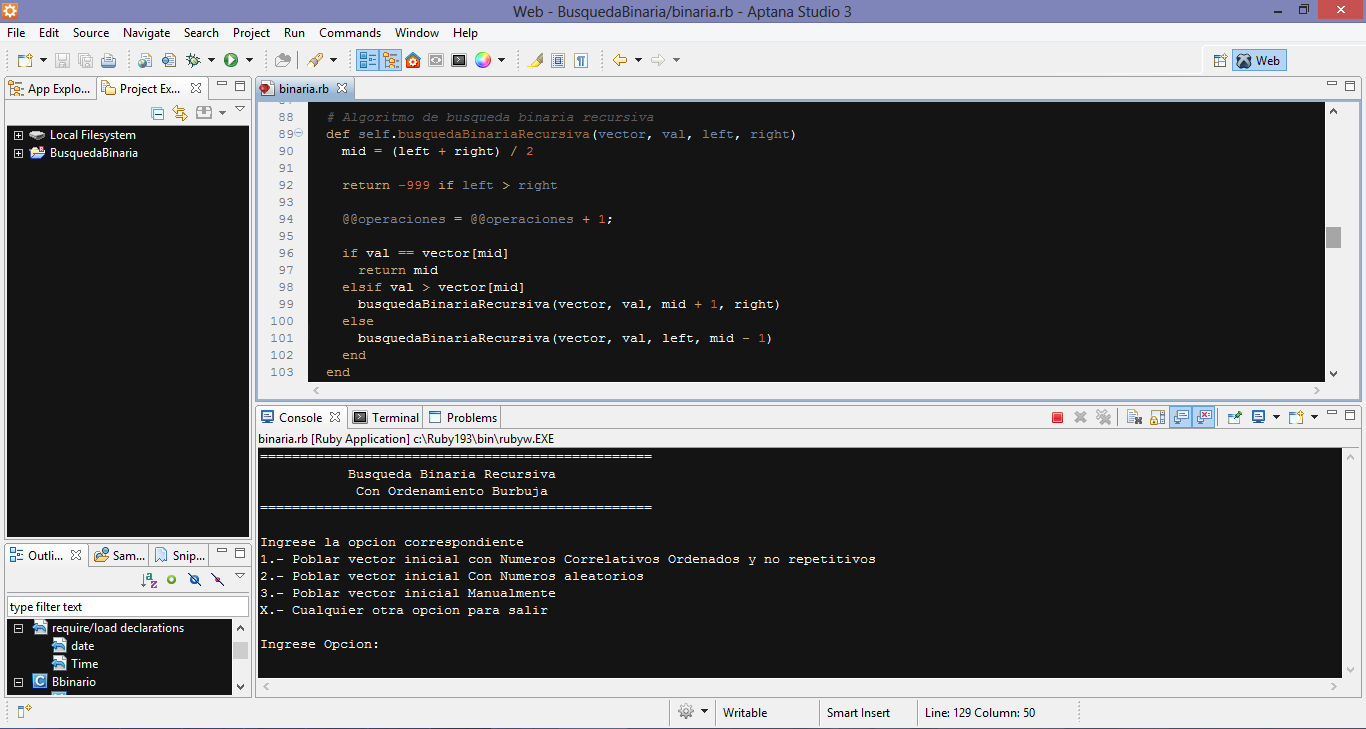
\includegraphics[scale=0.25]{Programa.png}
  				\caption{Pantallazo Aptana}
  				\label{fig:lls}
			\end{figure}	
	\end{frame}







\subsection{Ventajas} % A subsection can be created just before a set of slides with a common theme to further break down your presentation into chunks

		\begin{frame}
			\frametitle{Ventajas}
				\begin{center}
				Es un método eficiente siempre que el vector se encuentre ordenado.

                Proporciona un medio para reducir el tiempo requerido para buscar en una lista.
                Es más rápido debido a su recursividad, su mayor ventaja es con los archivos extensos.
                El código del procedimiento de está búsqueda es corto en comparación con las demás técnicas de búsquedas.

				\end{center}
		
		\end{frame}

		\begin{frame}
			\frametitle{Desventajas}
				
			\begin{center}
			El archivo debe estar ordenado y el almacenamiento de un archivo suele plantear problemas en la inserción y eliminación de elementos.

			No revisa todos los elementos del archivo.
			
			Debe conocerse el número de elementos. 

			\end{center}
		\end{frame}


\begin{frame}
			\frametitle{Aplicaciones}
				
			\begin{center}
			Partición Binaria del Espacio, usada en muchos videojuegos 3D para determinar que objeto necesita ser renderizado.

			Binary Tries, usada en casi todos los router de alta banda ancha para guardar las tablas de enrutamiento.

			
			Codificación Huffman, algoritmo usado para la compresión de datos, se utiliza en los formatos .jpeg y mp3. 

			\end{center}
		\end{frame}




\section{Conclusiones}
	\begin{frame}
		\frametitle{Conclusiones}
			\begin{itemize}[<+->]
				\item Se puede mejorar usando arboles autobalanceables, aunque estar asegurando minuciosamente puede añadir un costo considerable.
				\item No se nota la tendencia logaritmica de las inserciones debido a la complejidad lineal del recorrido.
			\item Otras Conclusiones
			\end{itemize}
	\end{frame}

	\begin{frame}
		\frametitle{Conclusiones}
		\begin{center}
\Huge
Fin\\
¿Alguna Pregunta?
		\end{center}	
	\end{frame}



\end{document} 


